% ==============================================================================
% SEZIONE 1 — INTRODUZIONE ALLE SNN E AI MODELLI DI NEURONE ARTIFICIALE
% ==============================================================================
\section[Introduzione alle SNN e modello LIF]{Introduzione alle SNN e modello LIF}
\label{sec:introduzione}

\subsection{Cos'è una Spiking Neural Network}
\label{subsec:paradigma}


Storicamente, i segnali biologici provenienti dagli elettrodi nei dispositivi elettronici vengono elaborati secondo l'architettura di von Neumann: il segnale viene campionato e convertito in digitale da un ADC, per poi passare ad un microcontrollore o ad un processore DSP. Questo approccio risulta inefficiente quando si devono elaborare segnali biologici lenti, sparsi nel tempo e caratterizzati da lunghi periodi di attività poco informativa (come l'elettroencefalogramma, i potenziali di campo locale o i potenziali d'azione extracellulari). Il continuo trasferimento di dati tra memoria e unità di calcolo comporta dei consumi energetici difficilmente sostenibili nei dispositivi impiantabili~\cite{qiao2015, moradi2018, bartels2025}.

Verso la fine degli anni ottanta, Carver Mead ha introdotto il concetto di ingegneria neuromorfica, che si basa sul progettare dei sistemi elettronici che emulano i principi computazionali del nostro sistema nervoso~\cite{indiveri2011}, sfruttando direttamente la fisica dei dispositivi. Un esempio sono le \emph{Spiking Neural Networks} (SNN), definite come le reti neurali di terza generazione~\cite{li2024}. Rispetto alle reti neurali tradizionali, in cui i neuroni si scambiano dei valori continui ad ogni ciclo di clock, nelle SNN l'informazione viene trasmessa con degli impulsi elettrici discreti chiamati \emph{spike} (come i potenziali d'azione biologici)~\cite{indiveri2011, li2024}. Ecco alcune caratteristiche delle SNN:
\begin{enumerate}
  \item L'informazione non è contenuta nell'ampiezza di un impulso, ma nell'istante di occorrenza e negli intervalli tra impulsi successivi (\emph{inter-spike interval}, ISI). Infatti, quando il segnale non mostra variazioni significative, la rete rimane quasi inattiva e i consumi si riducono drasticamente~\cite{indiveri2011, ronchini2023, bartels2025}.
  \item Il segnale viene elaborato in tempo reale mentre arriva, senza dover prima registrare in un buffer blocchi di campioni. Questo è possibile perché i circuiti hanno delle costanti di tempo dell'ordine dei millisecondi o decine di millisecondi, cioè gli stessi tempi dei segnali biologici~\cite{qiao2015, bartels2025}.
  \item Ogni neurone è collegato agli altri tramite le sinapsi, ovvero dei collegamenti su cui viaggiano gli spike. Ogni sinapsi ha un proprio peso, che viene memorizzato localmente, evitando così di dover leggere continuamente i pesi da una memoria esterna~\cite{qiao2015, moradi2018}.
  \item In un chip con migliaia di neuroni, è fisicamente impossibile collegare ogni neurone a tutti gli altri con dei fili dedicati. Per risolvere questo problema si usa il protocollo \emph{Address-Event Representation} (AER): ad ogni neurone viene assegnato un codice numerico univoco (quindi una specie di indirizzo); nel momento esatto in cui un neurone genera uno spike, invia il proprio indirizzo su un bus digitale condiviso, che lavora molto più velocemente dei tempi biologici (in nanosecondi) e permette di smistare gli spike ai neuroni destinatari usando pochissimi collegamenti fisici~\cite{indiveri2011, moradi2018}.
\end{enumerate}

\newpage

\subsection{Articoli di riferimento e criteri di scelta}
\label{subsec:perimetro}

Come richiesto dalla consegna, sono partito da 3 articoli di base: il primo è di Indiveri et al.\ (2011)~\cite{indiveri2011}, che illustra i principali circuiti in tecnologia CMOS usati per realizzare neuroni artificiali; presenta delle soluzioni complesse e molto vicine alla biologia, ma anche circuiti molto semplifici per ridurre area e consumi. Il secondo è lo studio di Qiao et al.\ (2015)~\cite{qiao2015}, che presenta ROLLS, un processore neuromorfico riconfigurabile che combina circuiti analogici e digitali, dotato di 256 neuroni e 128k sinapsi. Il terzo è il lavoro di Ronchini et al.\ (2023)~\cite{ronchini2023}, dedicato a NET-TEN, una rete neuromorfica analogica a bassissimo consumo progettata per rilevare gli eventi epilettici a partire dai potenziali di campo locale (LFP) registrati in vitro su tessuto cerebrale di topo.

Tra gli altri quattro articoli proposti nella consegna, ne ho scelti due per approfondire il tema della scalabilità e valutare i consumi reali. Il primo è di Moradi et al.\ (2018)~\cite{moradi2018}, che presenta il processore DYNAPs e affronta il problema di come gestire la memoria e lo smistamento degli spike quando la rete diventa grande; questo articolo è molto utile perché riporta nel dettaglio quanta area e quanta energia richiede ogni singola operazione sul chip. Il secondo è di Wu et al.\ (2026)~\cite{wu2026}, che propone NeuroSEED, un chip impiantabile che si occupa di: acquisire un segnale biologico da 32 canali; convertire il segnale in ingresso in spike; riconoscere dei potenziali d'azione e trasmettere via wireless dei dati verso l'esterno. Avere tutti questi blocchi sullo stesso chip permette di capire quanto consuma davvero un chip neuromorfico.

Ho deciso comunque di includere alla fine anche gli altri due paper della lista, perchè chiudono il cerchio sulle crisi epilettiche: l'articolo di Bartels et al.\ (2025)~\cite{bartels2025} usa il processore DYNAP-SE2 (evoluzione della famiglia DYNAP, che integra sullo stesso chip anche il circuito di acquisizione e di conversione del segnale in spike) per rilevare crisi epilettiche a partire da registrazioni EEG intracraniche umane; quello di Li et al.\ (2024)~\cite{li2024} rileva le crisi grazie a Xylo, un processore SNN interamente digitale con consumi inferiori al milliwatt, testato su registrazioni EEG di scalpo.

\subsection{Modelli matematici di un neurone artificiale}
\label{subsec:modelli_neurone}

Un neurone biologico è formato da tre parti principali:
\begin{itemize}
  \item I dendriti sono i rami d'ingresso, che ricevono i segnali provenienti dagli altri neuroni.
  \item Il soma è il corpo cellulare, che elabora i segnali in ingresso.
  \item L'assone è il canale d'uscita, lungo cui viaggiano gli spike emessi dal soma verso i neuroni successivi.
\end{itemize}

Gli spike che percorrono gli assoni dei neuroni raggiungono i punti di giunzione con i dendriti del neurone successivo, ovvero le sinapsi. Ciascuna sinapsi converte lo spike in arrivo in una piccola corrente elettrica, che può essere eccitatoria (EPSC) se tende ad attivare il neurone, oppure inibitoria (IPSC) se tende a frenarlo. Tutte le correnti ricevute si sommano nel soma caricando la membrana cellulare; se la tensione supera una certa soglia, il neurone genera a sua volta uno spike che viaggia verso i neuroni successivi~\cite{indiveri2011}. In letteratura esistono diversi modelli matematici che descrivono questo processo:

\begin{itemize}
  \item Modello di Hodgkin--Huxley (H--H): descrive in modo fedele come si comportano i canali presenti sulla membrana del neurone, cioè quei passaggi che si aprono e si chiudono in base alla tensione lasciando entrare e uscire ioni di sodio ($\mathrm{Na}^+$) e potassio ($\mathrm{K}^+$) per generare lo spike (insieme a una piccola corrente di perdita), usando un sistema di quattro equazioni differenziali non lineari~\cite{indiveri2011}. Il problema è che per realizzarlo su un chip richiede molti transistori, tanti parametri da regolare e molta area. Per questo è poco pratico per dispositivi impiantabili~\cite{indiveri2011}.
  \item Modello Leaky Integrate-and-Fire (LIF): è il modello più semplice ed efficiente dal punto di vista hardware. Descrive il neurone con tre semplici meccanismi: accumula nel tempo le correnti in ingresso facendo salire la tensione di membrana (\emph{integrate}), perde lentamente carica tornando verso il riposo se non arrivano nuovi stimoli (\emph{leaky}), e appena la tensione raggiunge una soglia prefissata emette uno spike e riporta subito la tensione al valore iniziale, di reset (\emph{fire})~\cite{indiveri2011, li2024}. Rispetto all'H-H, richiede pochissimi componenti circuitali e consuma molta meno energia.
  \item Modelli Integrate-and-Fire generalizzati: il modello LIF, essendo molto semplice, non riesce da solo a riprodurre alcuni comportamenti tipici dei neuroni reali, come l'adattamento della frequenza (Spike-Frequency Adaptation, SFA, cioè il fatto che sotto uno stimolo costante il neurone all'inizio spara veloce e poi rallenta) oppure il bursting (l'emissione di brevi raffiche di spike seguite da pause). Per ottenere questi comportamenti senza tornare alla complessità dell'H-H, si parte dal LIF e si aggiunge una seconda variabile che frena gradualmente il neurone mano a mano che spara. I tre modelli principali di questa famiglia presenti nei paper sono:
  \begin{enumerate}[label=(\alph*)]
    \item Modello di Izhikevich (2003): usa un'equazione con un termine quadratico ($\Vmem^2$) per descrivere la salita rapida dello spike assieme a una variabile lenta di recupero $U$ che riporta il neurone a riposo. Con pochi parametri riesce a imitare molti comportamenti reali ed è usato in NET-TEN~\cite{ronchini2023} e nei neuroni quadratici descritti in~\cite{indiveri2011};
    \item Modello Adaptive Exponential I\&F (AdEx-I\&F) di Brette e Gerstner (2005): modifica l'equazione del LIF aggiungendo un termine esponenziale che fa crescere molto rapidamente la tensione di membrana quando si avvicina alla soglia, e aggiunge una corrente di adattamento che frena il neurone dopo ogni spike. Si realizza con circuiti CMOS sottosoglia (circuiti DPI) ed è usato nei processori ROLLS~\cite{qiao2015}, DYNAPs~\cite{moradi2018} e DYNAP-SE2~\cite{bartels2025};
    \item Modello a soglia adattativa di Mihalas e Niebur (2009): la soglia di attivazione è variabile nel tempo, in funzione di $\Vmem$. Si realizza in CMOS con circuiti a capacità commutate, come analizzato in~\cite{indiveri2011}.
  \end{enumerate}
\end{itemize}

\subsection{Approfondimento sul modello Leaky Integrate-and-Fire (LIF)}
\label{subsec:modello_lif}

Dal punto di vista elettrico, la membrana cellulare del neurone viene modellata come un circuito RC parallelo (Figura~\ref{fig:lif_model}a): la capacità $C$ rappresenta lo strato lipidico capace di accumulare carica, mentre la resistenza di perdita $R$ modella i canali ionici passivi che scaricano la membrana verso il potenziale di riposo (nel circuito di Figura~\ref{fig:lif_model}a è la massa, cioè $\SI{0}{\volt}$, anche se in altri circuiti può essere fissato a una tensione di riposo dedicata~\cite{indiveri2011}). L'ingresso del circuito è la corrente totale $I(t)$ che arriva dalle sinapsi. Infatti, come si vede in Figura~\ref{fig:lif_model}b, ogni spike in ingresso viene moltiplicato per un peso e trasformato in una corrente con una propria costante di tempo, e infine tutte le correnti provenienti dai vari ingressi vengono sommate insieme~\cite{li2024}.

Applicando la legge di Kirchhoff alle correnti sul nodo superiore della Figura~\ref{fig:lif_model}a, la tensione $\Vmem(t)$ ai capi del parallelo $RC$ segue l'equazione differenziale~\cite{li2024}:
\begin{equation}
  RC \frac{\mathrm{d}\Vmem(t)}{\mathrm{d}t} = -\Vmem(t) + R\,I(t)
  \label{eq:lif_ode}
\end{equation}
dove $\tau_m = RC$ è la costante di tempo di membrana, che determina la memoria del neurone: se gli spike in ingresso arrivano troppo distanziati rispetto a $\tau_m$, la carica si consuma attraverso $R$ (che simula il \emph{leakage}) prima che il neurone raggiunga la soglia.

% --- FIGURA 1.1: Circuito equivalente LIF + Schema a blocchi (da Li et al., 2024) ---
\begin{figure}[tb]
  \centering
  \begin{subfigure}[b]{0.32\textwidth}
    \centering
    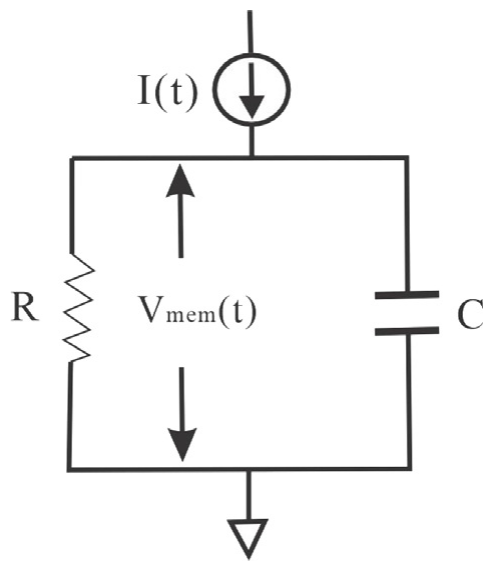
\includegraphics[height=3.8cm, keepaspectratio]{lif_circuit_li2024.png}
    \caption{}
  \end{subfigure}
  \hfill
  \begin{subfigure}[b]{0.64\textwidth}
    \centering
    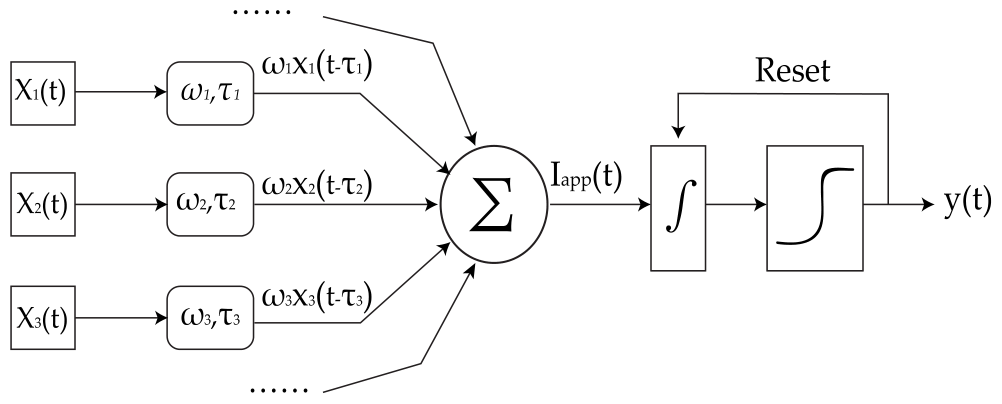
\includegraphics[height=3.8cm, keepaspectratio]{lif_block_li2024.png}
    \caption{}
  \end{subfigure}
  \caption[Principio di funzionamento del modello LIF]{(a) Circuito equivalente RC parallelo del LIF con corrente d'ingresso $I(t)$ e potenziale di membrana $\Vmem(t)$; (b) Schema a blocchi del neurone, da~\cite{li2024}.}
  \label{fig:lif_model}
\end{figure}

Quando la tensione di membrana $\Vmem(t)$ raggiunge la tensione di soglia $\Vthr$, il neurone genera uno spike e la tensione viene riportata subito a un valore inferiore, il potenziale di reset $V_{\mathrm{reset}}$~\cite{li2024} (che nei modelli più semplici coincide con il potenziale di riposo, ma in chip più avanzati come ROLLS può essere regolato separatamente~\cite{qiao2015}). Dopo aver generato uno spike, i neuroni possono rimanere anche inattivi per un breve intervallo di tempo, senza generare un nuovo impulso anche se continua ad arrivare corrente~\cite{indiveri2011, qiao2015}. Entrano in una specie di periodo refrattario. In pratica, aumentando la corrente in ingresso il neurone spara sempre più velocemente (secondo la sua curva caratteristica frequenza/corrente), ma il periodo refrattario fissa comunque una frequenza massima di sparo, che evita consumi eccessivi.

Come abbiamo visto in precedenza, esistono anche altri modelli di LIF più completi, che introducono una seconda variabile:
\begin{itemize}
  \item Il modello di Izhikevich introduce la variabile di recupero $U$. Valgono queste due equazioni:
  \begin{equation}
    \frac{\mathrm{d}\Vmem}{\mathrm{d}t} = 0{,}04\Vmem^2 + 5\Vmem + 140 - U + \Isyn,
    \qquad
    \frac{\mathrm{d}U}{\mathrm{d}t} = a(b\Vmem - U).
    \label{eq:izhikevich}
  \end{equation}
  Nella prima equazione il termine $-U$ agisce come un freno sulla crescita della tensione di membrana. Quando $\Vmem$ sale fino a raggiungere la soglia: il neurone spara l'impulso, la tensione viene riportata al valore di reset e la variabile $U$ aumenta di una certa quantità, frenando temporaneamente l'attività del neurone. Regolando $U$, si riescono a imitare molti comportamenti dei neuroni reali, come il bursting~\cite{indiveri2011, ronchini2023}.
  \item L'AdEx-I\&F invece utilizza una corrente di adattamento al posto di $U$ per frenare il neurone. Il termine quadratico che c'è nel modello di Izhikevich è sostituito da un termine esponenziale, e come vedremo nella Sezione~\ref{subsec:famiglie_neuroni}, si rivela molto utile perché si realizza facilmente sfruttando la fisica dei transistori CMOS sottosoglia~\cite{indiveri2011}.
\end{itemize}
